
\graphicspath{{./fig_Model/}}

%
\section{形状近似度による解析モデルの分類}
\label{sec:classification of model}
直交格子を用いる流体解析では,解析対象となる形状を直交格子上でどのように扱うかにより,計算のロバスト性,予測精度,計算時間,計算格子(解析モデル)の作りやすさなどの特性が異なります.一般には,\textbf{図\ref{fig:class model}}のように分類することができます\cite{CFDhandbook:03}.

\begin{figure}[htdp]
\begin{center}
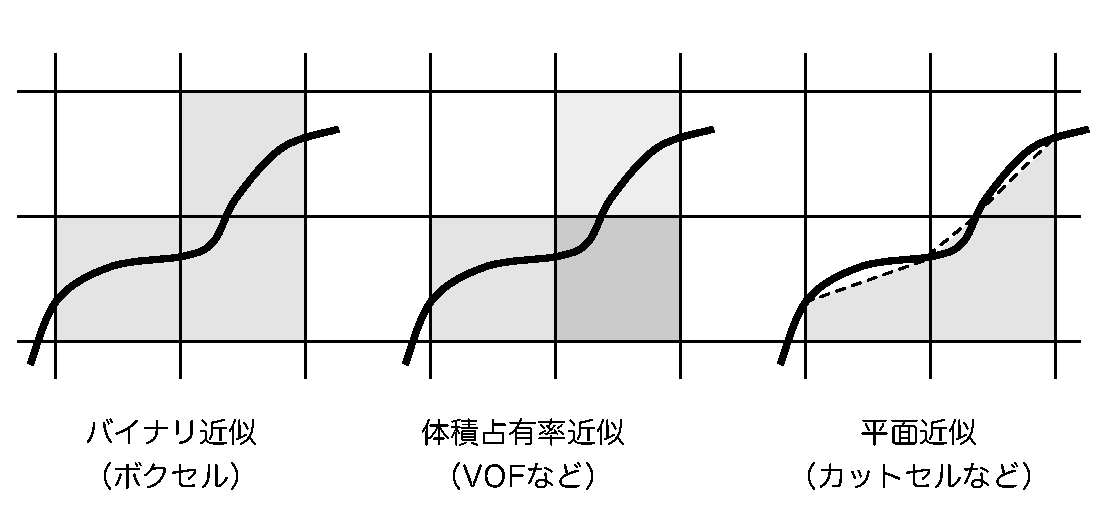
\includegraphics[width=11cm,clip]{classification.eps}
\caption{直交格子における形状近似度の分類}
\label{fig:class model}
\end{center}
\end{figure}

%
\subsection{Binary Voxel}
Binary Voxel\index{Binary Voxel}モデルは,\textbf{図\ref{fig:Eport binary voxel}}に示すように立方体のセル要素単位で形状を表現する解析モデルです.
物体の形状近似としては最も簡単であり,モデル作成時のロバスト性に大きな利点があります.

\begin{figure}[htbp]
\begin{center}
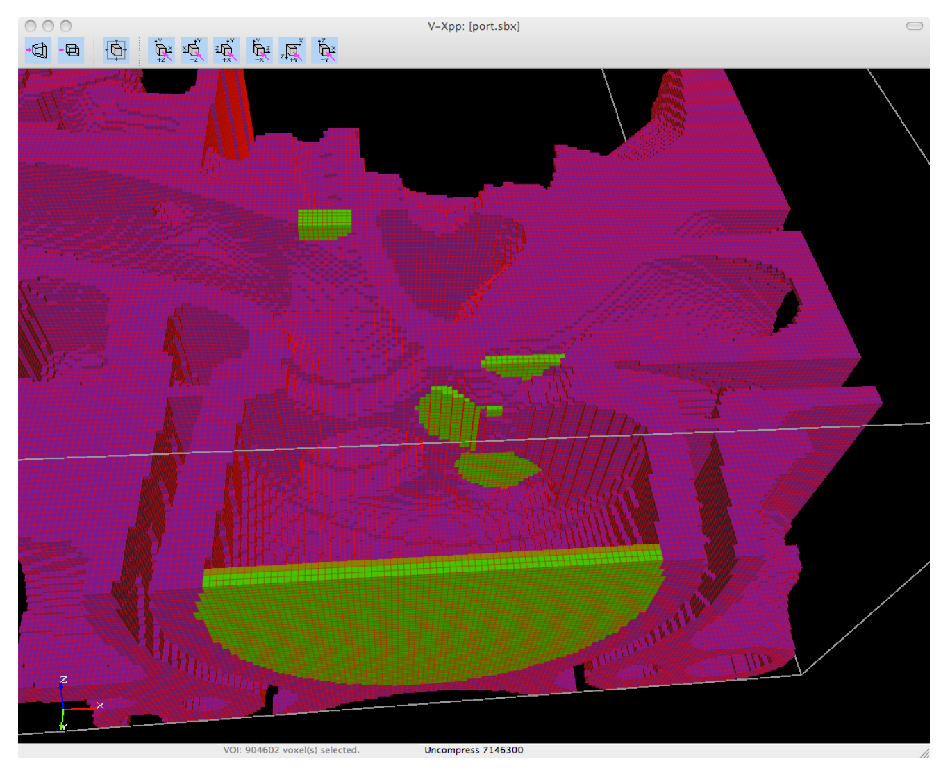
\includegraphics[width=8cm,clip]{eport.eps}
\end{center}
\caption{バイナリボクセルによる機械部品の形状表現}
\label{fig:Eport binary voxel}
\end{figure}

%
\subsection{体積率モデル}
Binary Voxelの形状近似度を改善する方法の一つで,セル内における流体の占有率を考慮した計算をする場合に利用します.
FFV-Cソルバーでは,圧力損失部などの境界条件の実装に用いています.

%
\subsection{距離情報モデル}
Binary Voxelでは形状が階段状に近似されるため,計算精度が不足する場合があります.そこで,格子の定義点から物体表面までの距離を用いて流束計算を行うスキームを用います.


%
\section{ポリゴンによる境界条件の指定}

FFV-Cソルバーでは,解析する形状を表すポリゴンにIDを与え,このIDとパラメータファイルに記述された境界条件情報を結びつけ,境界条件を設定するしくみになっています.

下記のファイルは,計算に利用する解析モデルのポリゴン情報ファイルの内容です.
Eng\_BlockとExhaustの2つのグループがあります.

{\small
\begin{program}
$ cat polylib.tp

Polylib {

  Eng_Block {
    class_name = "PolygonGroup"
    filepath ="./geom_scaled/Eng_Block.stl"
    movable = "false"
    id = 3
    label = "Fe-heat_src_1"
  }

  Exhaust {
    class_name = "PolygonGroup"
    filepath = "./geom_scaled/Exhaust.stl"
    movable = "false"
    id = 4
    label = "Fe-heat_src_2"
  }
}
\end{program}
}

\noindent ここでは,Eng\_Blockには,Fe-heat\_src\_1のラベルが付与されています.
このラベルは媒質を表しており,
参照される媒質IDは,Medium\_Tableタグによって次のように指定されます.

{\small
\begin{program}
Medium_Table {
  Medium[@] { // Eng_Block
    type                 = "Solid"
    label                = "Fe-heat_src_1"
    Density              = 7870.0
    Specific_Heat        = 442.0
    Thermal_Conductivity = 80.3
  }
  Medium[@] { // Exhaust
    type                 = "Solid"
    label                = "Fe-heat_src_2"
    Density              = 7870.0
    Specific_Heat        = 442.0
    Thermal_Conductivity = 80.3
  }
}
\end{program}
}

媒質IDの指定についての詳細は,\hyperlink{tgt:medium_table}{Medium\_Table}セクションを参照してください.

Eng\_BlockとExhaustの各ポリゴン部分が境界条件を表しますが,LocalBoundaryで具体的な境界条件の種類を指定します.

{\small
\begin{program}
BC_Table {

  LocalBoundary {

    BC[@] {
      class                    = "HeatTransfer_SN"
      alias                    = "Eng_Block"
      neighbor_medium          = "air-100c"
      Surface_Temperature      = 100.0
      Ref_Temp_Mode            = "Bulk_Temperature"
      vertical_laminar_alpha   = 0.59
      vertical_laminar_beta    = 0.25
      vertical_turbulent_alpha = 0.1
      vertical_turbulent_beta  = 0.3333333
      vertical_Ra_critial      = 1.0e9
      lower_laminar_alpha      = 0.27
      lower_laminar_beta       = 0.25
      lower_turbulent_alpha    = 0.27
      lower_turbulent_beta     = 0.25
      lower_Ra_critial         = 1.0e9
    }

    BC[@] {
      class                    = "HeatTransfer_SN"
      alias                    = "Exhaust"
      neighbor_medium          = "air-100c"
      Surface_Temperature      = 500.0
      Ref_Temp_Mode            = "Bulk_Temperature"
      vertical_laminar_alpha   = 0.59
      vertical_laminar_beta    = 0.25
      vertical_turbulent_alpha = 0.1
      vertical_turbulent_beta  = 0.3333333
      vertical_Ra_critial      = 1.0e9
      lower_laminar_alpha      = 0.27
      lower_laminar_beta       = 0.25
      lower_turbulent_alpha    = 0.27
      lower_turbulent_beta     = 0.25
      lower_Ra_critial         = 1.0e9
    }
\end{program}
}

\pagebreak
%
\section{形状データからの解析モデルの作成手順}


%% 
\section{組み込み例題}
\hypertarget{tgt:intrinsic model}{組み込み例題}は,FFV-Cソルバーに組み込み済みの解析モデルです.
プログラムに組み込まれた解析モデルを用いることにより,解析モデルを作成しなくても計算ができます.
ただし,\textbf{表\ref{tbl:intrinsic problems}}に示すような簡単な形状のモデルに限られます.
各モデルに固有のパラメータは,Parameter $>$ Intrinsic\_Exampleセクションで指定します.

\begin{table}[htdp]
\caption{組み込み例題クラス}
\begin{center}
\small
\begin{tabular}{lll}\toprule
組み込みモデル名 & 利用クラス & 説明\\ \midrule
%Users & IP\_Users & ユーザ問題(解析モデルファイルを指定する場合)\\ \hline
%Back\_Step & IP\_STEP & バックステップ流れのモデル\\
%Cylinder & IP\_CYLINDER & 角柱と円柱周りの流れのモデル\\
%Duct & IP\_Duct & 円形と正方形のダクト流れのモデル\\
%Parallel\_Plate\_2D & IP\_PPLT2D & 二次元平行平板のモデル(Poiseuille流れ,Couette流れなど)\\
Performance\_Test & IP\_PMT & 性能測定を行うためのモデル(三次元立方体キャビティフローと同じ問題設定)\\
%Polygon & IP\_Polygon & 距離情報スキームを用いる場合に,入力するポリゴンファイル名とDomainInfoの\\
% & & 指定だけで計算するモデル\\
Rectangular & IP\_Rect & 計算領域が矩形で,かつ単一媒質のモデル\\
%SHC1D & IP\_SHC1D & 一次元の熱伝導問題のモデル\\ 
\bottomrule
\end{tabular}
\end{center}
\label{tbl:intrinsic problems}
\end{table}

%
\begin{comment}
\subsection{IP\_STEPクラス}
バックステップ流れを計算するクラスです.
\textbf{図\ref{fig:ip_backstep}}と\textbf{表\ref{tbl:ip_backstep}}および\textbf{表\ref{tbl:ip_backstep_ID}}に示すパラメータで計算空間を構成します.
計算領域は,Domain\_Infoで指定するVoxelSize,VoxelPitch,VoxelOriginで決まります.

ドライバー部分については,Ductクラスの設定を参照してください.

\begin{figure}[htdp]
\begin{center}
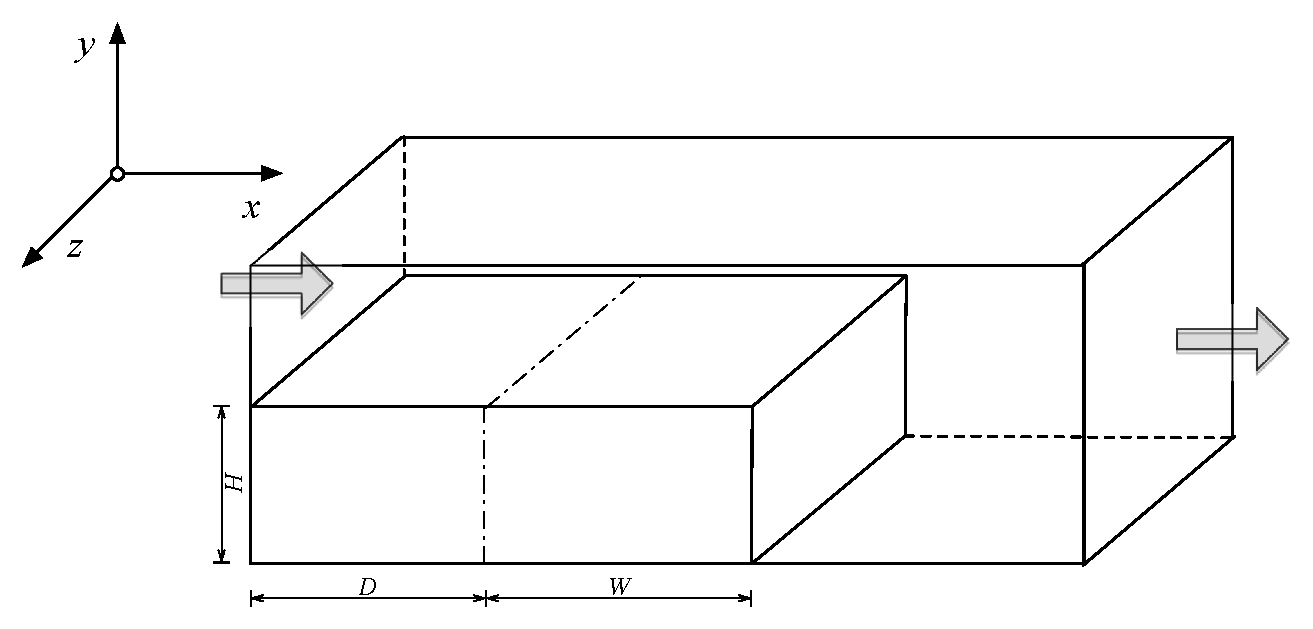
\includegraphics[width=14cm,clip]{Backstep.eps}
\end{center}
\caption{バックステップ流れの計算モデル.}
\label{fig:ip_backstep}
\end{figure}

\begin{table}[htdp]
\small
\caption{バックステップ問題のパラメータ.}
\begin{center}
\begin{tabular}{ll}\toprule
記号 & パラメータ\\ \midrule
Mode & 2D $|$ 3D\\ \hline
Width ($W$) & ステップの$x$方向の幅\\
Height ($H$) & ステップの$y$方向の高さ\\
Driver ($D$) & ドライバー部分の長さ($>0.0$でドライバあり,=0.0の場合ドライバーなし)\\
\bottomrule
\end{tabular}
\end{center}
\label{tbl:ip_backstep}
\end{table}

\begin{table}[htdp]
\small
\caption{バックステップ問題のID番号.}
\begin{center}
\begin{tabular}{ll}\toprule
ID & 属性\\ \midrule
1 & 流体\\
2 & 固体\\
3 & ドライバ部分の流体\\
4 & ドライバ流出面(流体)\\
\bottomrule
\end{tabular}
\end{center}
\label{tbl:ip_backstep_ID}
\end{table}

境界条件として,X-方向に流入,またはドライバ境界,X+方向は流出条件,Y-方向は壁面,Y+方向は壁面またはスリップ条件,Z$\pm$方向は壁面か周期境界を与えて計算します.二次元の問題を解く場合には,Mode=2Dを指定,VoxelSizeはkmax=3として,Z方向は周期境界条件を与えてください.
\end{comment}

%
\begin{comment}
\subsection{IP\_CYLINDERクラス}
二次元と三次元の円柱・角柱まわりの流れを計算するクラスです.
\textbf{図\ref{fig:ip_cylinder}}と\textbf{表\ref{tbl:ip_cylinder}}に示すパラメータで計算空間を構成します.
断面形状は,円柱と角柱をShapeで指定します.それぞれの断面形状で指定するパラメータが異なります.
柱は$xy$平面の$z-$方向に接しています.これを基準に長さのパラメータを指定してください.

二次元の問題を解く場合には,Mode=2Dを指定,VoxelSizeはkmax=3としてください.この場合,パラメータ$W$は無視されます.

\begin{figure}[htdp]
\begin{center}
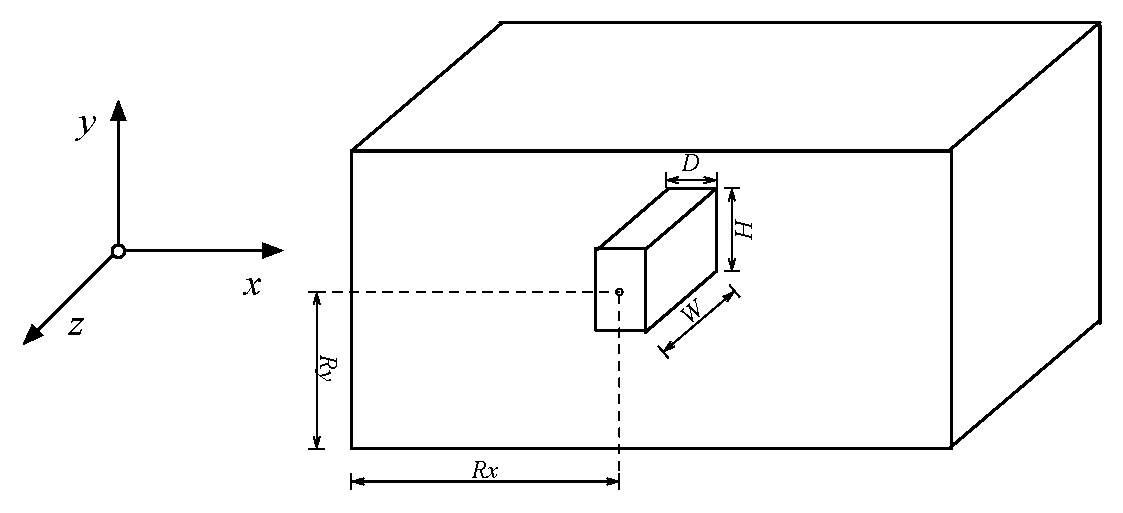
\includegraphics[width=14cm,clip]{Cylinder.eps}
\end{center}
\caption{円柱・角柱モデルの計算空間.}
\label{fig:ip_cylinder}
\end{figure}

\begin{table}[htdp]
\small
\caption{柱状物体の指定パラメータ}
\begin{center}
\begin{tabular}{ll}\toprule
記号 & パラメータ\\ \midrule
Mode & 2D $|$ 3D\\ 
Shape & Rectangular $|$ Circular\\ \hline
$D$ & 角柱を指定時の角柱の幅\\
$H$ & 角柱を指定時の角柱の高さ\\
$R$ & 円柱を指定時の半径\\
$W$ & 柱の$z$軸方向の長さ\\
$R_x$ & 柱の中心位置と$x$方向領域境界からの距離\\
$R_y$ & 柱の中心位置と$y$方向領域境界からの距離\\
\bottomrule
\end{tabular}
\end{center}
\label{tbl:ip_cylinder}
\end{table}
\end{comment}

%
\begin{comment}
\subsection{IP\_Ductクラス}
\textbf{図\ref{fig:ip_duct}}のような円形と矩形のダクト流れを計算するモデルで,周期境界条件を用います.
流入面には,流れを発達させる機能をもつドライバー部分を指定することができます.

断面形状は,正方形または円形をShapeで指定し,
流入部の方向をDirectionで指定します.
ドライバー部は,Directionで指定した方向にドライバ部分が配置されます.
ドライバー部分を指定する場合には,Driverにその長さ$D$を指定してください.
$D=0.0$の場合には,ドライバー無しの指定になります.

\begin{figure}[htdp]
\begin{center}
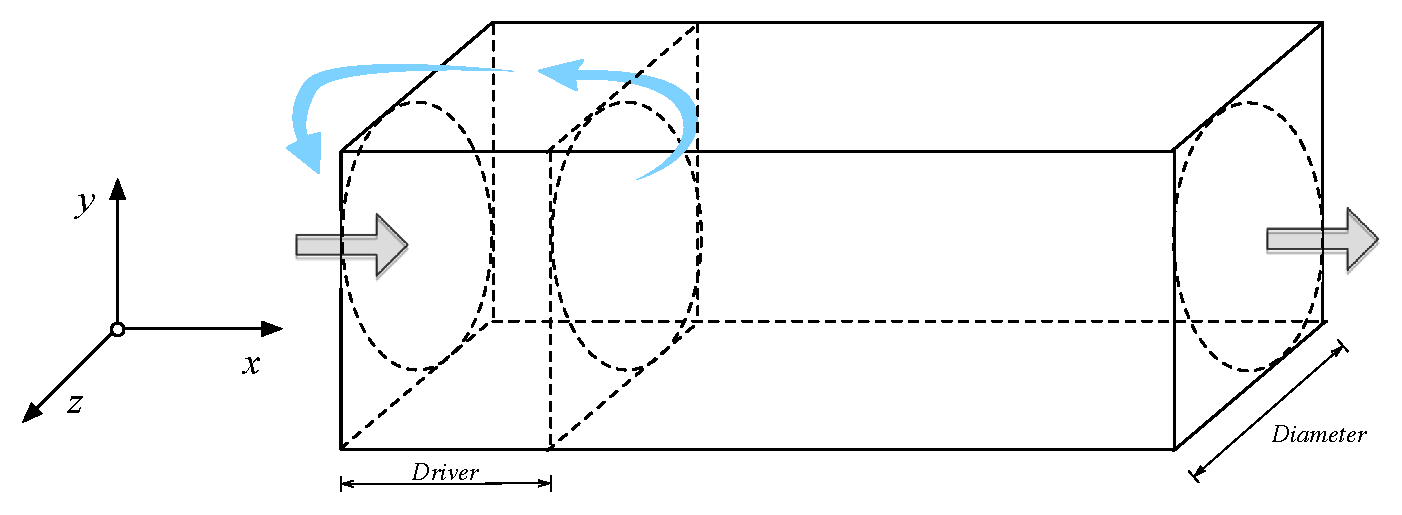
\includegraphics[width=16cm,clip]{Duct.eps}
\end{center}
\caption{ダクトの計算空間.$X-$方向にドライバ部を設置した場合.}
\label{fig:ip_duct}
\end{figure}

\begin{table}[htdp]
\small
\caption{ダクトの指定パラメータ}
\begin{center}
\begin{tabular}{ll}\toprule
記号 & パラメータ\\ \midrule
Shape & Rectangular $|$ Circular\\ \hline
Diameter & 正方形または円の直径\\
Direction & 周期境界と流入の方向(X\_minus, X\_plus, Y\_minus, Y\_plus, Z\_minus, Z\_plus)\\
Driver & ドライバー部分の長さ($>0.0$でドライバあり,=0.0の場合ドライバーなし)\\
\bottomrule
\end{tabular}
\end{center}
\label{tbl:ip_duct}
\end{table}
\end{comment}


%%
\subsection{IP\_PMTクラス}
FFV-Cソルバーの基本的性能を測定するための例題クラスです.
三次元立方体の空間内のキャビティフローを解きます.
性能測定モードとなり,圧力反復の収束判定は行わず,反復回数は固定となります.
また,初期化時のファイル出力が抑制されます.



%%
\begin{comment}
\subsection{IP\_PPLT2Dクラス}
二次元の平行平板間の流れを計算するためのクラスです.
\textbf{図\ref{fig:pplate2d}}のように辺長比が2:1の二次元空間を表現します.
z方向には3セルを設けており,単純な周期境界条件を用いて二次元を近似しています.
したがって,VoxelSizeでは\lq\lq kmax=3 \rq\rq を指定し,分割数imaxとjmaxの比は2:1となるように指定します.
空間格子幅は,x方向とy方向で同じ(直交等間隔)としています.

計算領域内部は単一媒質(セルID=1)が設定されています.
この例題は,パラメータ指定\lq\lq Unit\_of\_input\_parameter\rq\rq に無次元を指定します.

\begin{figure}[htdp]
\begin{center}
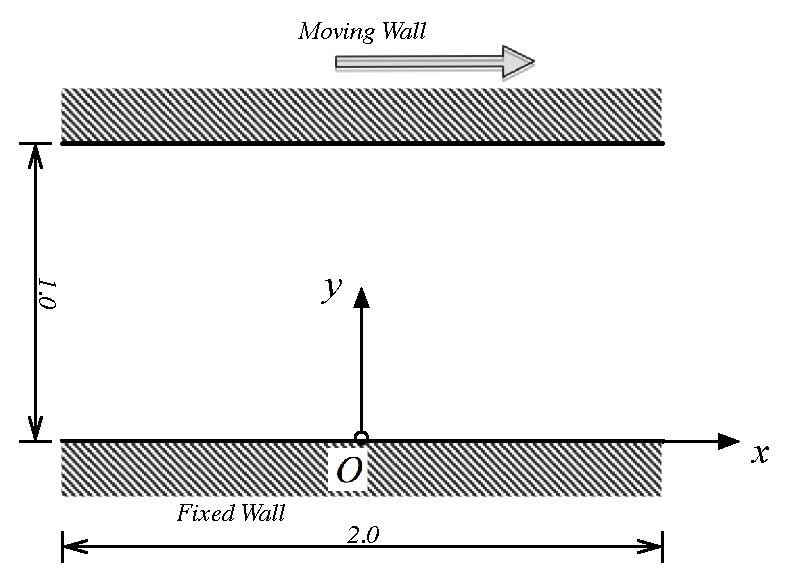
\includegraphics[width=8cm,clip]{PPLT2D.eps}
\end{center}
\caption{二次元平行平板間の計算空間.}
\label{fig:pplate2d}
\end{figure}
\end{comment}


%%
\subsection{IP\_Rectクラス}
IP\_Rectクラスは三次元の矩形の計算領域を表現するクラスです.
計算領域は,次のようにDomainファイルで指定します.
ここでは,各方向の格子幅を指定し,基点座標と計算領域の大きさを指定しています.


{\small
\begin{program}
DomainInfo {
  Global_origin   = (-0.5, -0.5, -0.5   )
  Global_region   = (1.0,  1.0,  1.0    )
  Global_pitch    = (1.5625e-02, 1.5625e-02, 1.5625e-02)
  ActiveSubDomain_File = ""
}
\end{program}
}


\begin{figure}[htdp]
\begin{center}
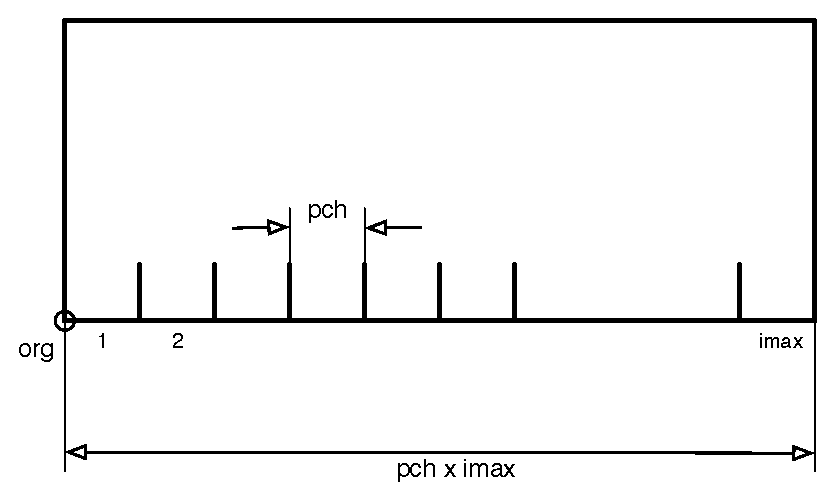
\includegraphics[width=9cm,clip]{rect.eps}
\caption{Rectangularクラスのパラメータ設定}
\label{fig:rect intrinsic class}
\end{center}
\end{figure}


\begin{table}[htdp]
\caption{Intrinsic\_Exampleタグで設定可能なパラメータ}
\begin{center}
\small
\begin{tabular}{lll}\toprule
指定パラメータ & 指定値 & 意味\\ \midrule
Check\_Even & Yes $|$ No & 分割数が偶数であるかどうかをチェックする\\
Fluid\_Medium & Medium\_Tableのラベル名 & 流体の媒質\\
Solid\_Medium & Medium\_Tableのラベル名 & 固体の媒質\\
\bottomrule
\end{tabular}
\end{center}
\label{tbl:rect parameter}
\end{table}

\textbf{表\ref{tbl:rect parameter}}のパラメータは,IP\_Rectクラスに固有の設定項目で,Parameter $>$ Intrinsic\_Exampleセクションで指定します.

{ \small
\begin{program}
  Intrinsic_Example {
    fluid_medium = "air"
    solid_medium = "fe"
    check_even = "yes"
  }
\end{program}
}

上記のパラメータ設定では,分割数の偶数チェックを行い,Medium\_TableにおいてAir,Feのラベル名で指定されている物性値を,それぞれ流体と固体として参照しています.



%
\begin{comment}
\subsection{IP\_Polygonクラス}
XMLファイルで,\lq\lq Steer > Solver\_Property > Shape\_Approximation\rq\rq でDistance\_Infoを指定すると,距離情報を用いたスキームで計算します.
この\hypertarget{tgt:polygon_class}{IP\_Polygonクラス}は,入力するポリゴンファイルと,DomainInfoで指定する計算領域情報のみで計算を行うモデルテンプレートです.ポリゴンファイル名は,\lq\lq Steer > Polygon\_File\rq\rq で指定します.
\end{comment}

%
\begin{comment}
\subsection{IP\_SHC1Dクラス}
\textbf{図\ref{fig:HC1D}}に示すような片持ちはりの熱伝導問題を一次元の定常熱伝導問題として解くためのクラスです.
この問題には厳密解があり,厳密解と計算結果を比較することにより予測精度の確認ができます.

\begin{figure}[htdp]
\begin{center}
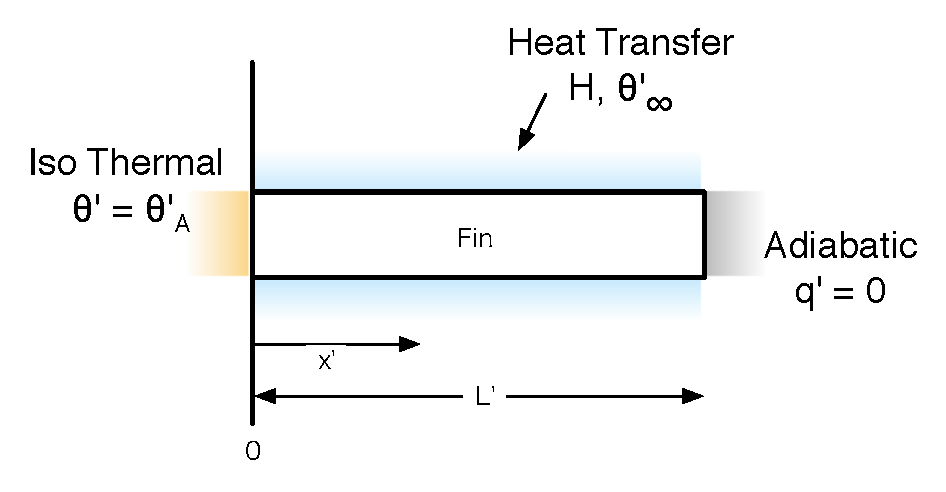
\includegraphics[width=9cm,clip]{1DHC.eps}
\end{center}
\caption{一次元定常熱伝導問題の模式図}
\label{fig:HC1D}
\end{figure}


計算領域は\textbf{図\ref{fig:HC model}}に示すようにx軸方向に放熱フィンをとり,y,z方向には5つだけセルを設けます.
領域の設定パラメータとして,x方向の分割数をimaxにより与えます.
放熱フィンを5分割したい場合には,imax=7を設定します.
その他の方向は$\mathrm{jmax=kmax=5}$で固定です.

例題と解析結果の詳細については,例題集をご覧ください.

\begin{figure}[htdp]
\begin{minipage}{0.47\hsize}
\begin{center}
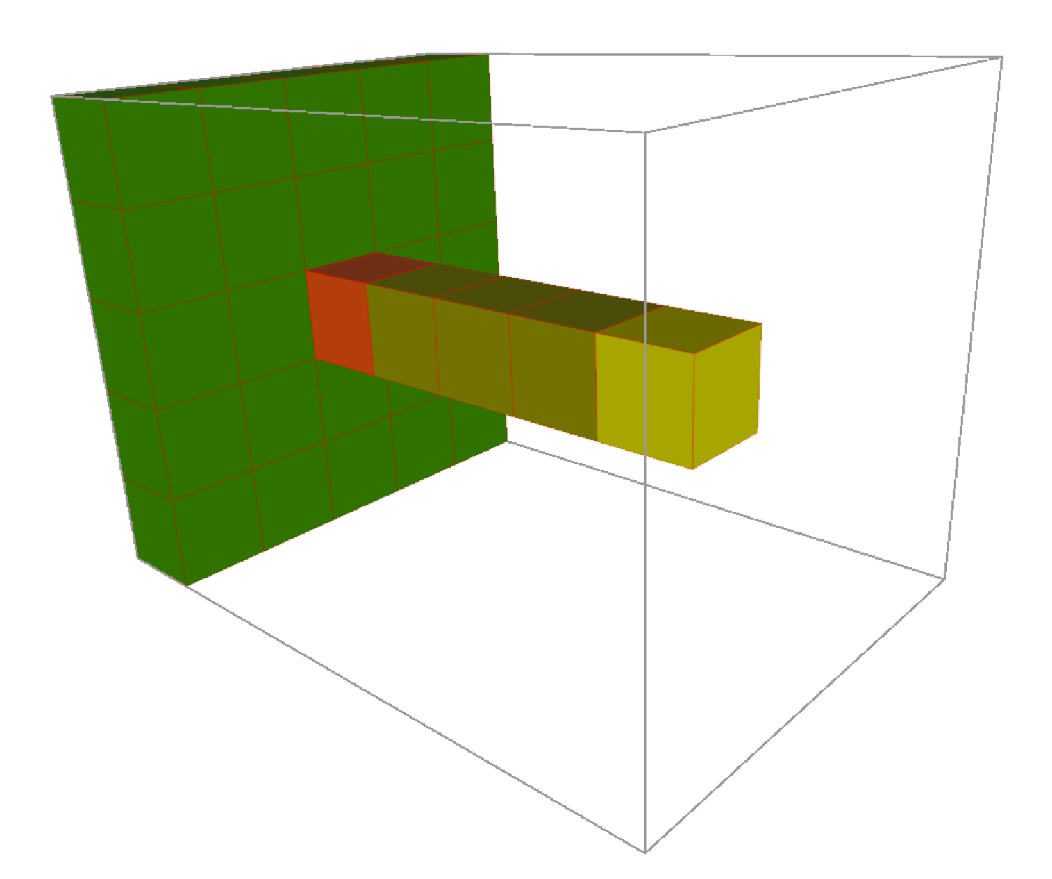
\includegraphics[height=5cm,clip]{model_iso.eps}
\end{center}
\end{minipage}
\begin{minipage}{0.47\hsize}
\begin{center}
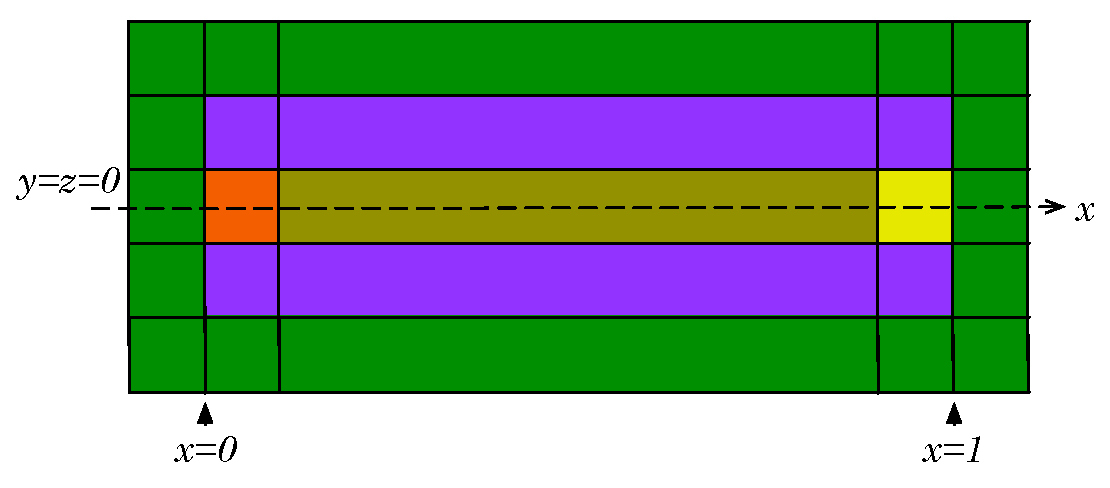
\includegraphics[height=3.5cm,clip]{dimension.eps}
\end{center}
\end{minipage}
\caption{一次元熱伝導問題を計算するための片持ち梁の三次元モデルとセルID (分割数が$7\times5\times5$の場合)}
\label{fig:HC model}
\end{figure}
\end{comment}

\pagebreak
% 
\section{例題}
ソースファイルのExampleディレクトリに含まれる\hypertarget{tgt:samples}{例題}について説明します.
提供される例題は,組み込みモデルや簡単なボクセルモデルを同梱した例題群で,
基本的な流れやソルバーの検証のために用意されています.


\begin{table}[htdp]
\caption{組み込み例題}
\begin{center}
\small
\begin{tabular}{lll} \toprule
Example & Class & Comment\\ \midrule
Cavity flow 3D (Cube) & IP\_Rect & 三次元立方体キャビティフロー\\
LDC112  & IP\_Rect & Guermondの実験に対応する辺長が1:1:2のキャビティフロー\\ 
%Duct 3D & IP\_Duct3D & ダクト流れ\\ 
PMT & IP\_PMT & 性能測定を行うための例題(三次元立方体キャビティフローの例題と同じ)\\
\bottomrule
\end{tabular}
\end{center}
\label{tbl:example at glance}
\end{table}


\begin{table}[htdp]
\caption{サンプル例題}
\begin{center}
\small
\begin{tabular}{lll} \toprule
Example & Comment\\ \midrule
%Dragon & Asian Dragon周りの流れ\\
%Heated Plate & 流体中の平板からの放熱\\
%SHC1D & 熱伝導計算の解析解との比較\\ \bottomrule
\end{tabular}
\end{center}
\label{tbl:exercise}
\end{table}

